% Chapter Template

\chapter{Results \& Comparison} % Main chapter title

\label{Chapter5} % Change X to a consecutive number; for referencing this chapter elsewhere, use \ref{ChapterX}


To verify the correctness of the new implementation, it will be compared to the original implementation from \parencite{klampfl_maass_2013}, starting with toy models to prove equal behavior on the smallest possible level and proper functioning of individual properties like plasticity and lateral inhibition (Section \ref{sec:toy_models}). After that, the tested network's size will be increased until the parameters of the full-scale model described in Figure 4 of \parencite{klampfl_maass_2013} are reached (Section \ref{sec:full_scale}).

\section{Toy Models} \label{sec:toy_models}
%\begin{table}[]
%\begin{tabular}{|l|lllllll|}
%\hline
%Test & Grid size   & $K$ & lateral inhibition & STDP & STP & Rate & Input rate \\
%\hline
%1A   & $1\times 2$ & 1   & Off                & On   & Off & 50   & 60         \\
%1B   & $1\times 2$ & 1   & Off                & On   & Off & 100  & 2          \\
%2    & $1\times 2$ & 2   & On                 & On   & Off & 50   & 20         \\
%3    & $1\times 2$ & 2   & On                 & On   & On  & 50   & 20         \\  
%\hline
%\end{tabular}
%\end{table}
%%%%%%%%%%%%%%%%%%%%%%%%%%%%%%%%%%%%%%%%%%%%%%%%%%%%%%%%%%%%%%%%%%%%%%%%%%%%%%%%%%%%%%%
\subsection{Baseline Test} \label{ssec:baseline_test}
\begin{figure}[htbp]
    \centering
    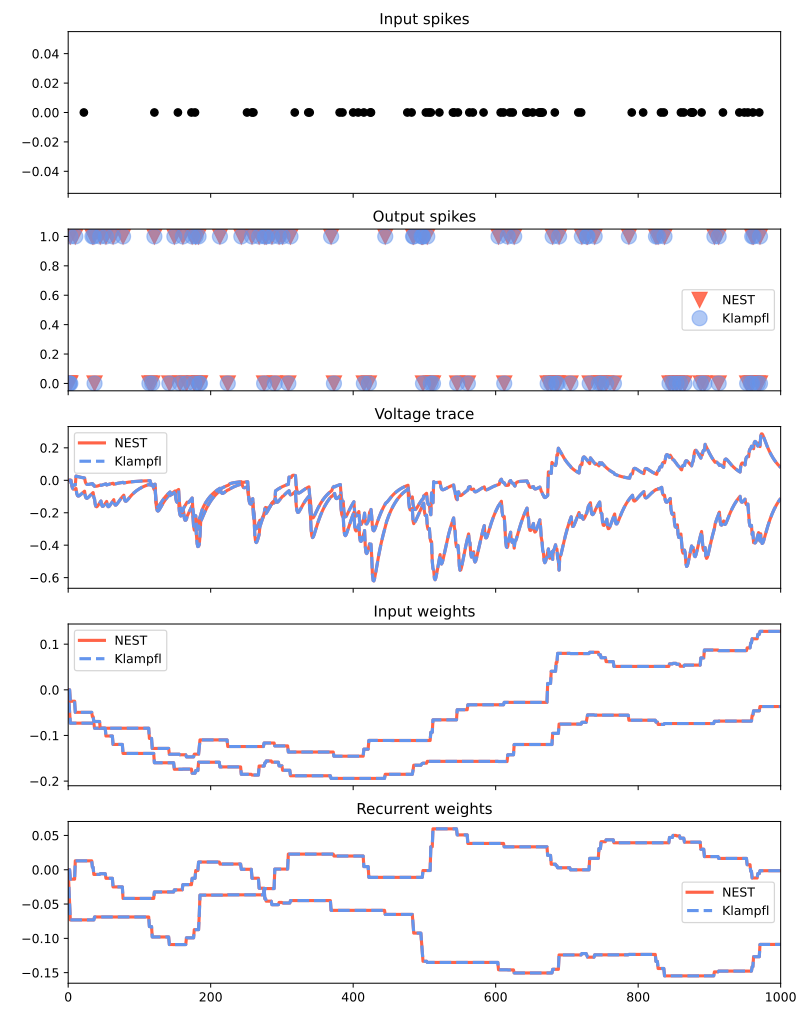
\includegraphics[width=\columnwidth]{Figures/joint_tm_2wta1.png}
    \caption{Toy Model: Test of $1\times 2$ WTA grid with $k=1$ and one input channel for \SI{1}{\second}. Input and output spikes are fixed at \SI{60}{\hertz} and \SI{50}{\hertz}. STP is disabled.}
    \label{fig:joint_tm_2wta1_A}
\end{figure}
\begin{figure}[htbp]
    \centering
    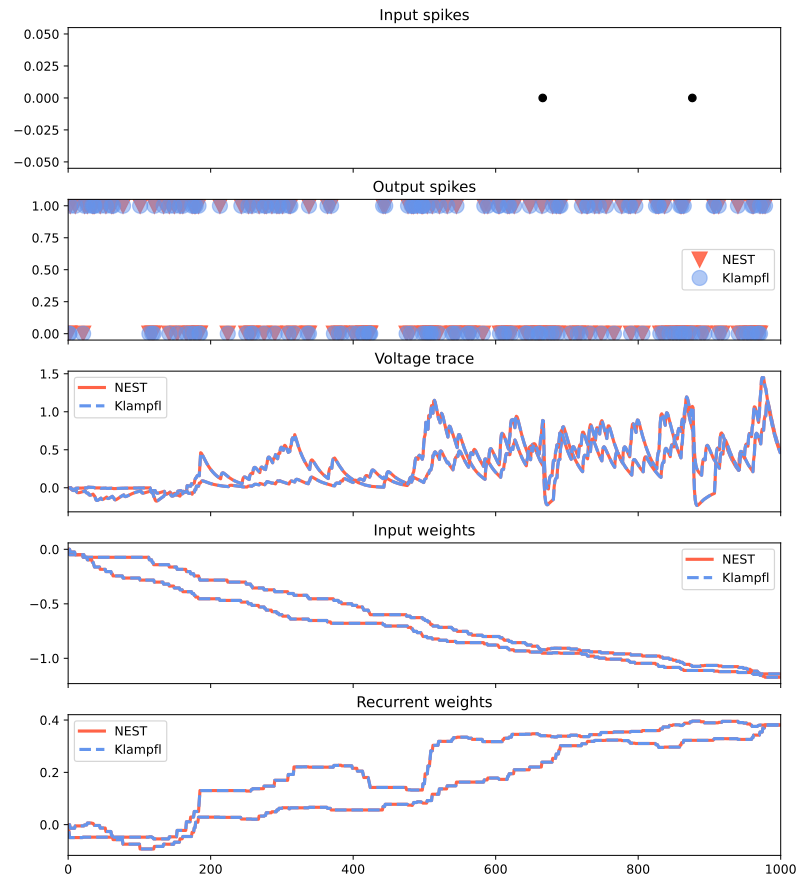
\includegraphics[width=\columnwidth]{Figures/joint_tm_2wta1_B.png}
    \caption{Toy Model: Test of $1\times 2$ WTA grid with $k=1$ and one input channel for \SI{1}{\second}. Input and output spikes are fixed at \SI{2}{\hertz} and \SI{100}{\hertz}. STP is disabled.}
    \label{fig:joint_tm_2wta1_B}
\end{figure}
To start off, a minimal network of grid size $1\times2$, in which each WTA contains just one neuron will be tested for a singular input source over \SI{1000}{\milli\second}. The WTA size is set to $1$ to bypass the effect of lateral inhibition. STP is also disabled, leaving only STDP as a dynamic network property to test. The purpose of this test is to prove the equal behavior of both implementations, which is why the embedded stochastic firing behavior of both implementations is turned off and replaced with predefined spike times, both for neuron in- and output, which were generated randomly and set to be identical for both programs externally. For the input firing rate and neuron firing rate \SI{50}{\hertz} and \SI{60}{\hertz} were chosen respectively.\\
The results of this test can be seen in Figure \ref{fig:joint_tm_2wta1_A}, where the pre-generated in- and output spikes are visualized along with the weights of the incoming and recurrent synaptic connections within the network and the resulting membrane potential ("Voltage trace").\\
From these results, we can conclude that since the plotted traces for both programs do not deviate from one another, the behavior of STDP and membrane potential in this context without lateral inhibition and STP is identical for original and replication. And since the membrane potential is computed as the sum of the EPSP scaled by the respective synaptic weights, this implies also that the EPSPs are identical. But more can be deduced from the same test setup by changing the firing rates to \SI{2}{\hertz} for input and \SI{100}{\hertz} for recurrent output spiking (Figure \ref{fig:joint_tm_2wta1_B}). With neither STP nor lateral inhibition at work, weights can switch signs depending on the rate of the external input and output firing rates of the neurons. This also shows that Dale's principle (described in Chapter \ref{Chapter2}) 
is not preserved when using STDP and STP disabled, since both inhibition and excitation of neurons by the same entities are possible, which is proven by the voltage traces of Figure \ref{fig:joint_tm_2wta1_A} and \ref{fig:joint_tm_2wta1_B} developing toward both positive and negative values. That being said, Dale's principle is not enforced in this model in any way, i.e. the weights are not bound to a specific interval during learning.

%%%%%%%%%%%%%%%%%%%%%%%%%%%%%%%%%%%%%%%%%%%%%%%%%%%%%%%%%%%%%%%%%%%%%%%%%%%%%%%%%%%%%%%
\subsection{Scaled WTA Test}
\label{ssec:lateral_inhibition_test}
\begin{figure}[htbp]
    \centering
    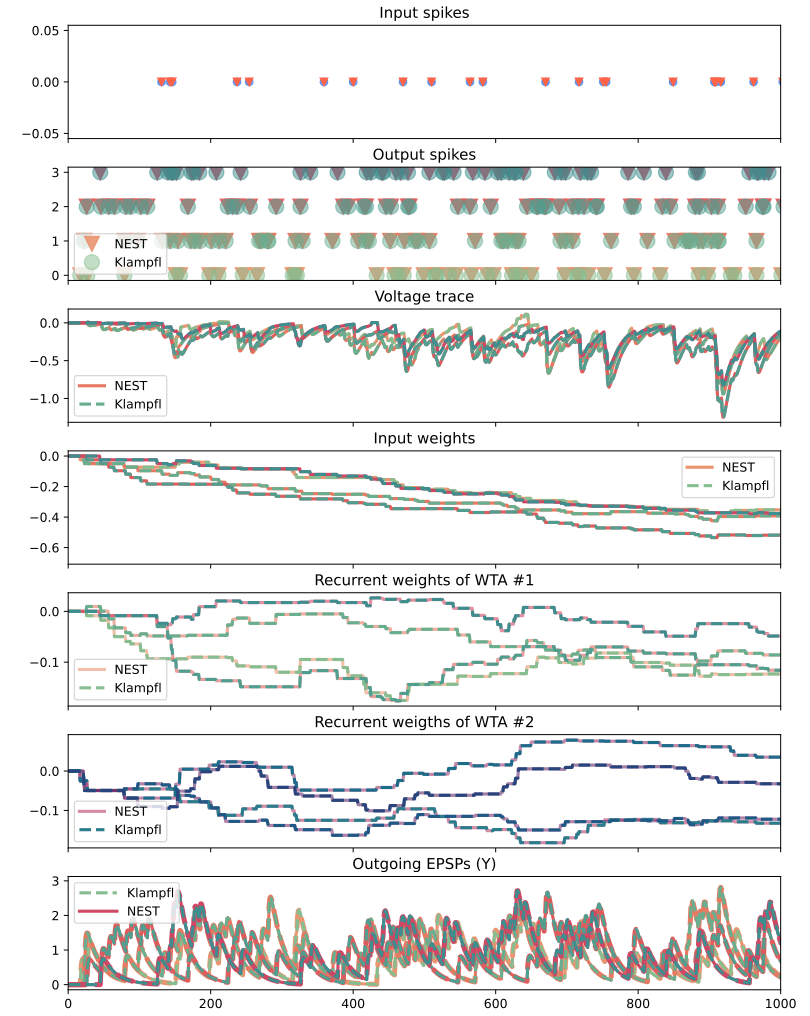
\includegraphics[width=\columnwidth]{Figures/joint_tm_2wta2.png}
    \caption{Toy Model: Test of $1\times 2$ WTA grid with $k=2$ and one input channel for \SI{1}{\second}. Input and output spikes are fixed at \SI{20}{\hertz} and \SI{50}{\hertz}. STP is disabled.}
    \label{fig:joint_tm_2wta2}
\end{figure}
The second test (Figure \ref{fig:joint_tm_2wta2}) serves as an intermediate test for later comparison. It increases the WTA size from $1$ in the last test to $2$ and also adds a plot for EPSPs.
This setup allowed testing the \texttt{rate\_connection\_instantaneous} along with the rate normalization in general, more specifically if the values of the \texttt{rate\_fraction}s were computed correctly. Most parameters are taken from \ref{ssec:baseline_test}, except for the fixed firing rates, which were set to \SI{50}{\hertz} and \SI{20}{\hertz} for recurrent and input firing rate respectively. Original and replication still produce identical results. 

%%%%%%%%%%%%%%%%%%%%%%%%%%%%%%%%%%%%%%%%%%%%%%%%%%%%%%%%%%%%%%%%%%%%%%%%%%%%%%%%%%%%%%%
\subsection{STP Test} \label{ssec:stp_test}
\begin{figure}[htbp]
    \centering
    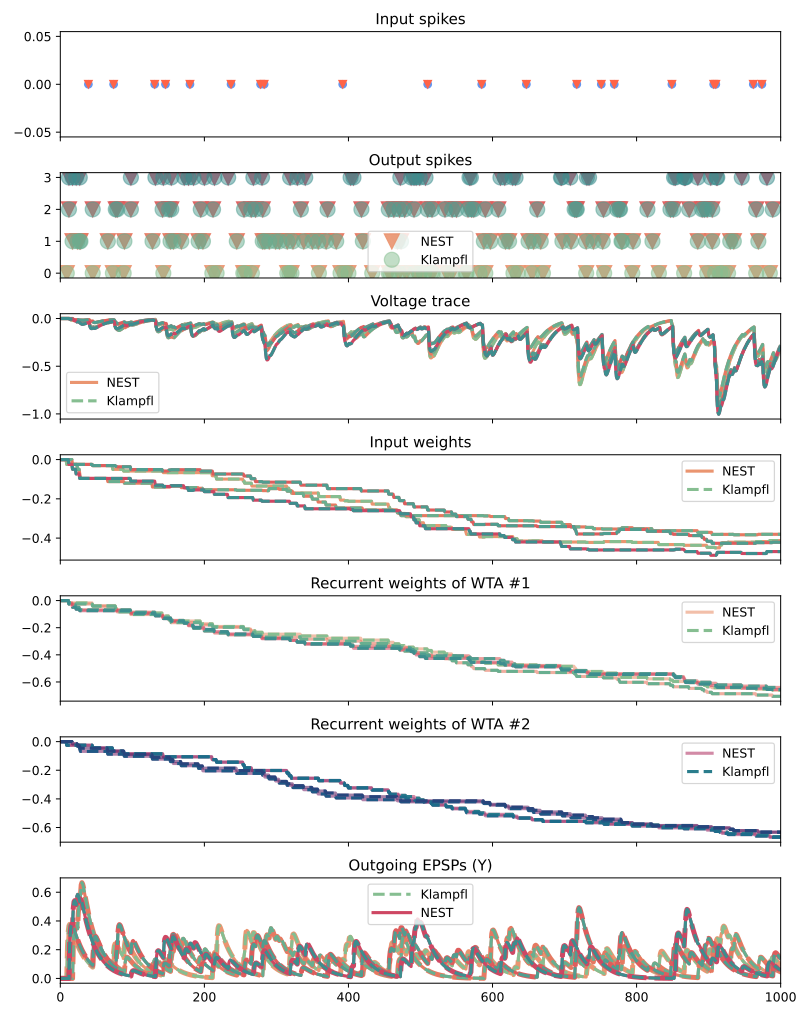
\includegraphics[width=\columnwidth]{Figures/joint_tm_2wta2_stp.png}
    \caption{Toy Model: Test of $1\times 2$ WTA grid with $k=2$ and one input channel for \SI{1}{\second}. Input and output spikes are fixed at \SI{20}{\hertz} and \SI{50}{\hertz}. STP is enabled.}
    \label{fig:joint_tm_2wta2_stp}
\end{figure}
For the next test, all parameters stay the same as in \ref{ssec:lateral_inhibition_test}, except for STP which is now enabled, producing the plot in Figure \ref{fig:joint_tm_2wta2_stp} and allowing a comparison of network behavior with and without STP in combination with Figure \ref{fig:joint_tm_2wta2}. Notice that the addition of STP makes the recurrent weights diverge to the negative range and stabilizes the membrane potential to the negative range, whereas the voltage trace without STP contained positive valued outliers. However, weight and voltage adjustments are just the secondary effects of the EPSP being directly affected by STP, vastly reducing its maximum excitability.


%%%%%%%%%%%%%%%%%%%%%%%%%%%%%%%%%%%%%%%%%%%%%%%%%%%%%%%%%%%%%%%%%%%%%%%%%%%%%%%%%%%%%%%%%%
%%%%%%%%%%%%%%%%%%%%%%%%%%%%%%%%%%%%%%%%%%%%%%%%%%%%%%%%%%%%%%%%%%%%%%%%%%%%%%%%%%%%%%%%%%
%%%%%%%%%%%%%%%%%%%%%%%%%%%%%%%%%%%%%%%%%%%%%%%%%%%%%%%%%%%%%%%%%%%%%%%%%%%%%%%%%%%%%%%%%%
\section{Full Scale Network} \label{sec:full_scale}
\subsection{Formation of Assemblies}
With the accuracy of the implementation proven for all major components of the model, it can now be compared if the full-scale models still produce the same results. For testing larger models, fixing random numbers between implementations becomes prohibitive, meaning that these tests' results are not expected to be identical and should rather show the same qualitative behavior. For the following tests, networks with the following properties will be compared in Figure \ref{fig:nest_full_scale} and \ref{fig:legacy_full_scale}:\\
\begin{table}[h!]
\begin{tabular}{|ll}
Grid size            & $10\times 5$                                       \\
WTA size range       & [2; 10]                                            \\
\#Input channels     & 100                                                \\
Training time        & \SI{100}{\second}                                  \\
Testing time         & \SI{3}{\second}                                    \\
\#Patterns           & 1                                                  \\
Noise duration range & [\SI{300}{\milli\second}; \SI{500}{\milli\second}] \\
Pattern duration     & \SI{300}{\milli\second}                       
\end{tabular}
\end{table}

\begin{figure}[htbp]
    \centering
    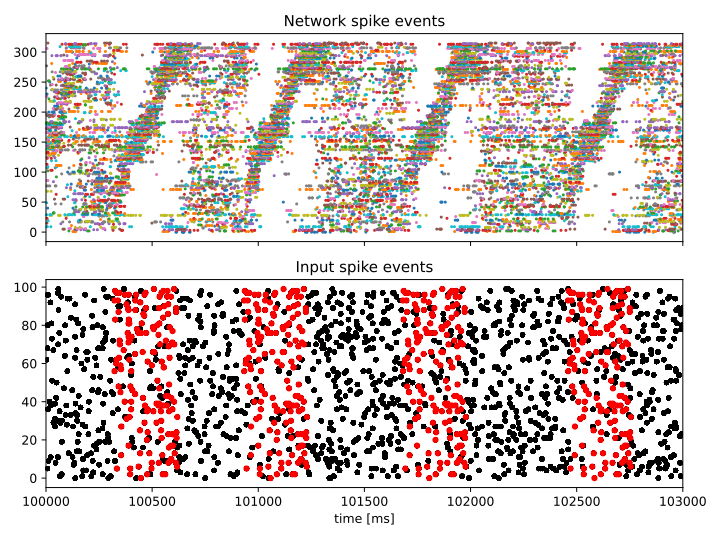
\includegraphics[width=\columnwidth]{Figures/nest_full_scale.png}
    \caption{Full-scale Network: NEST \SI{3}{\second} test after \SI{100}{\second} training}
    \label{fig:nest_full_scale}
\end{figure}
\begin{figure}
    \centering
    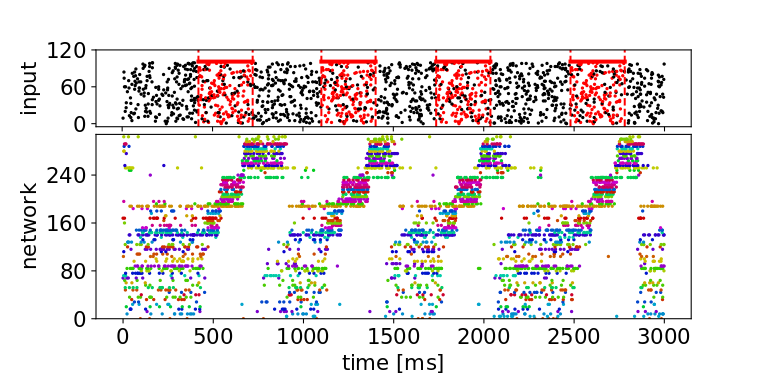
\includegraphics[width=\columnwidth]{Figures/legacy_full_scale.png}
    \caption{Full-scale Network: Legacy \SI{3}{\second} test after \SI{100}{\second} training. Only 100 neurons plotted to reduce clutter in network spikes plot.}
    \label{fig:legacy_full_scale}
\end{figure}

\subsection{Necessity of Variance Tracking}
During testing of the original implementation, it was also found that variance tracking was in fact crucial to the learning capabilities of the model as can be seen in Figure \ref{fig:variance_tracking_comparison}. This figure shows the results of two \SI{3}{\second} testing runs of the network each following a \SI{100}{\second} training phase. During the training phase a network of grid size $10\times 5$ and $k\in[2; 10]$ with $100$ input channels was fed with a \SI{5}{\hertz} of either pattern input (shown in red) or noise input (black), with \SI{2}{\hertz} of noise additionally laid over each pattern phase. As can clearly be seen, if variance tracking is enabled, assemblies of neurons with similar spike characteristics emerge as a consequence of pattern input, while disabling variance tracking prevents the formation of such assemblies. From this follows that variance tracking as described in \parencite{nessler_et_al_2013} is a requirement for learning in \parencite{klampfl_maass_2013}, while the STDP rule from Equation \ref{eqn:stdp_real} alone does not appear to be able to make such learning possible.\\
This phenomenon can also be replicated in the NEST implementation as demonstrated in Figure \ref{fig:nest_full_scale_no_variance_tracking}.
\begin{figure}[htbp]
    \centering
    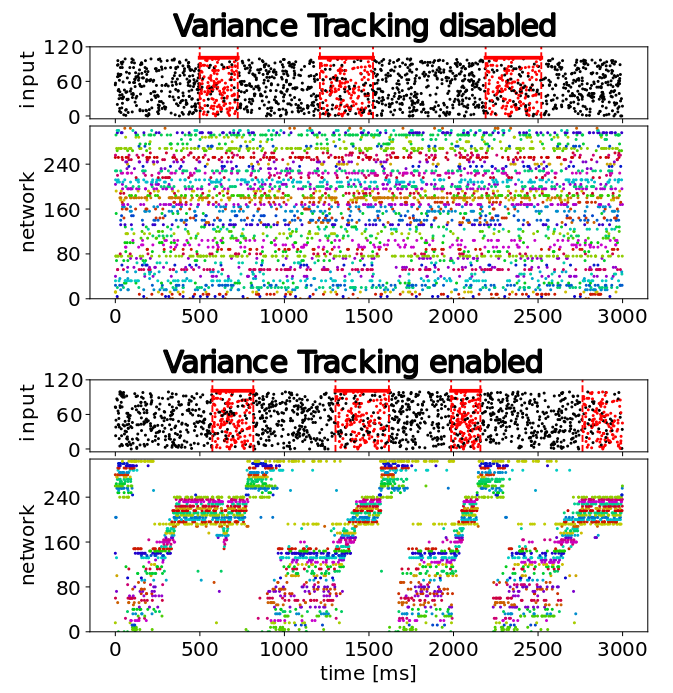
\includegraphics[width=0.8\columnwidth]{Figures/variance_tracking_comparison.png}
    \caption{Full-scale Network: Legacy \SI{3}{\second} test after \SI{100}{\second} simulation with and without variance tracking}
    \label{fig:variance_tracking_comparison}
\end{figure}
\begin{figure}[htbp]
    \centering
    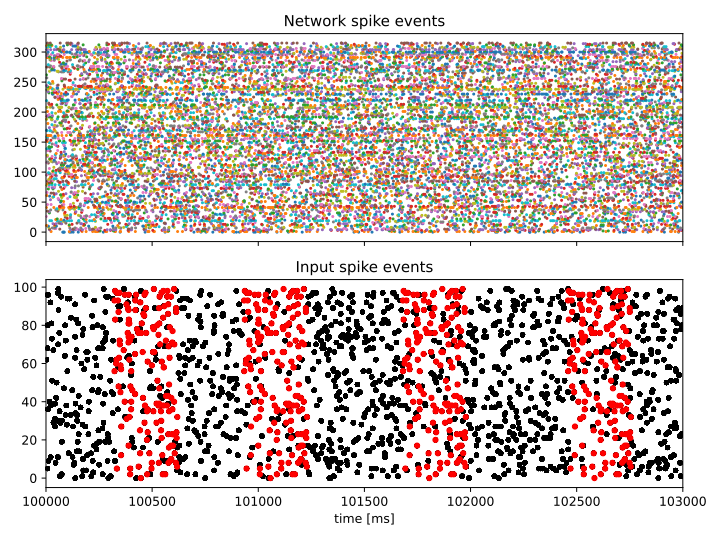
\includegraphics[width=0.85\columnwidth]{Figures/nest_full_scale_no_variance_tracking.png}
    \caption{Full-scale Network: NEST \SI{3}{\second} test after \SI{100}{\second} training without variance tracking}
    \label{fig:nest_full_scale_no_variance_tracking}
\end{figure}

\subsection{Necessity of STP}
For the following test, STP will be turned off for testing its effect on long-term network spike behavior. In \parencite{klampfl_maass_2013} Figure 6A a similar test is conducted with a slightly different testing setup in the "without depressing synapses" panel, which means nothing else than "without STP". As can be seen when comparing Figure \ref{fig:nest_full_scale_no_stp} to the Figure in \parencite{klampfl_maass_2013}, the behavior without STP is comparable in both cases.
\begin{figure}[htbp]
    \centering
    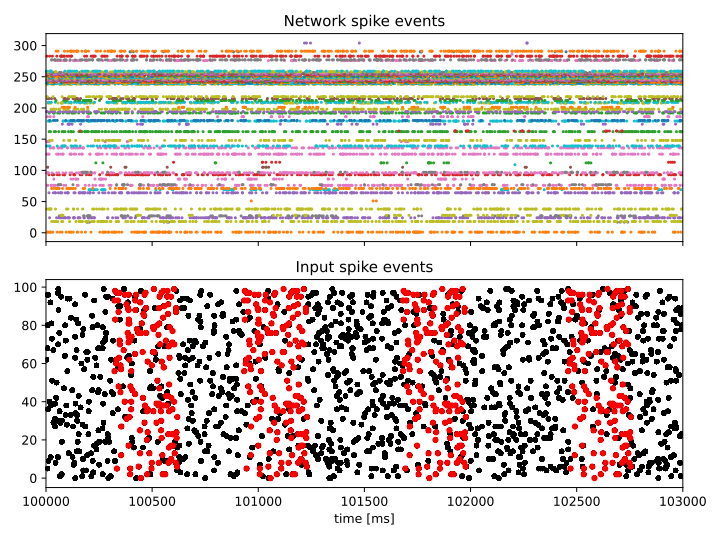
\includegraphics[width=\columnwidth]{Figures/nest_full_scale_no_stp.png}
    \caption{Full-scale Network: NEST \SI{3}{\second} test after \SI{100}{\second} training without STP}
    \label{fig:nest_full_scale_no_stp}
\end{figure}

\subsection{Performance Benchmarking}
An important asset of the NEST implementation that has not yet been mentioned is its vastly superior performance. This is an effect of the more efficient simulation kernel of NEST, whereas the version of Klampfl and Maass simulates stepwise and uses matrix multiplication for calculation. In the table below the real-time factors of simulations for both implementations are benchmarked for the full-scale model task from Section \ref{sec:full_scale}. The hardware used for benchmarking is a Lenovo YOGA 730-15IWL Notebook with 16GB of memory, an Intel Core i7-8565U CPU with 8 cores, and running Ubuntu 22.04 LTS. The original implementation will use all cores while the NEST implementation here only uses 6 cores.
\begin{table}[htbp]
\centering
\begin{tabular}{|l|l|l|}
\hline
       & Real-time factor & Simulation Time                                     \\ \hline
NEST   & 0.7362           & \SI{73.63}{\second}                                 \\
Legacy & 41.83            & \SI{69}{\minute} \SI{43}{\second} = \SI{4183}{\second} \\ \hline
\end{tabular}
\end{table}

\section{Further Experiments}
\begin{figure}[htbp]
    \centering
    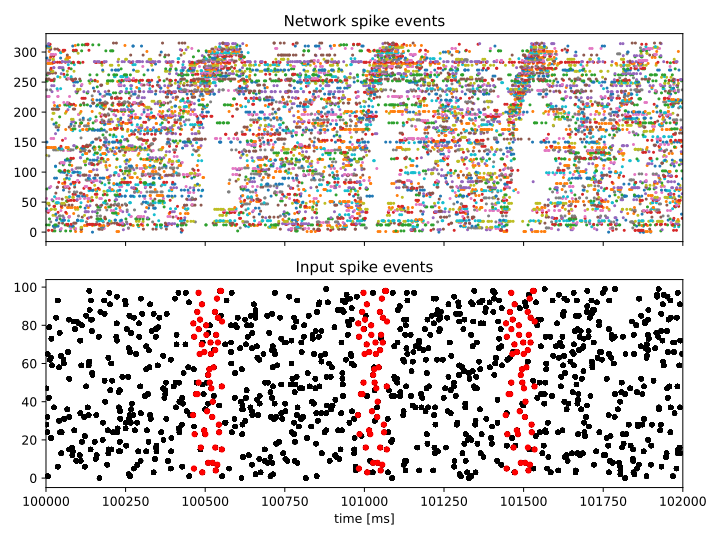
\includegraphics[width=\columnwidth]{Figures/nest_experiment_100ms.png}
    \caption{Pattern duration set to \SI{100}{\milli\second}. Grid size $10\times 5$ with $k\in[2;10]$ and 100 input channels. Input rate of \SI{5}{\hertz} with additional \SI{2}{\hertz} during pattern presentation. \SI{2}{\second} test after \SI{100}{\second} training.}
    \label{fig:nest_experiment_100ms}
\end{figure}
To test a few of the boundaries of the replicated model, the pattern duration was varied to examine the assembly formation under these conditions. Figure \ref{fig:nest_experiment_100ms} shows the results of a pattern duration of \SI{100}{\milli\second} and Figure \ref{fig:nest_experiment_900ms} shows the result of a pattern duration of \SI{900}{\milli\second}. The first visible difference between short and long duration is the size of the formed assembly. Where the long pattern activates almost the entire network over time, the shorter pattern activates a much smaller assembly. This also comes with different levels of assembly distinction. The short pattern causes a clear phase of inactivity for a part of the network, while the longer pattern already activates the whole network, preventing parts of it to become inactive and therefore impeding learning.
\\ \ \\
In both cases conclusions are deducible: Too long patterns cannot be learned by the network because they overstimulate it, preventing assemblies of reduced activity during pattern presentation to form. Too short patterns on the other hand can only excite small assemblies, to the point where they will not have a noticeable effect at all.
\begin{figure}[htbp]
    \centering
    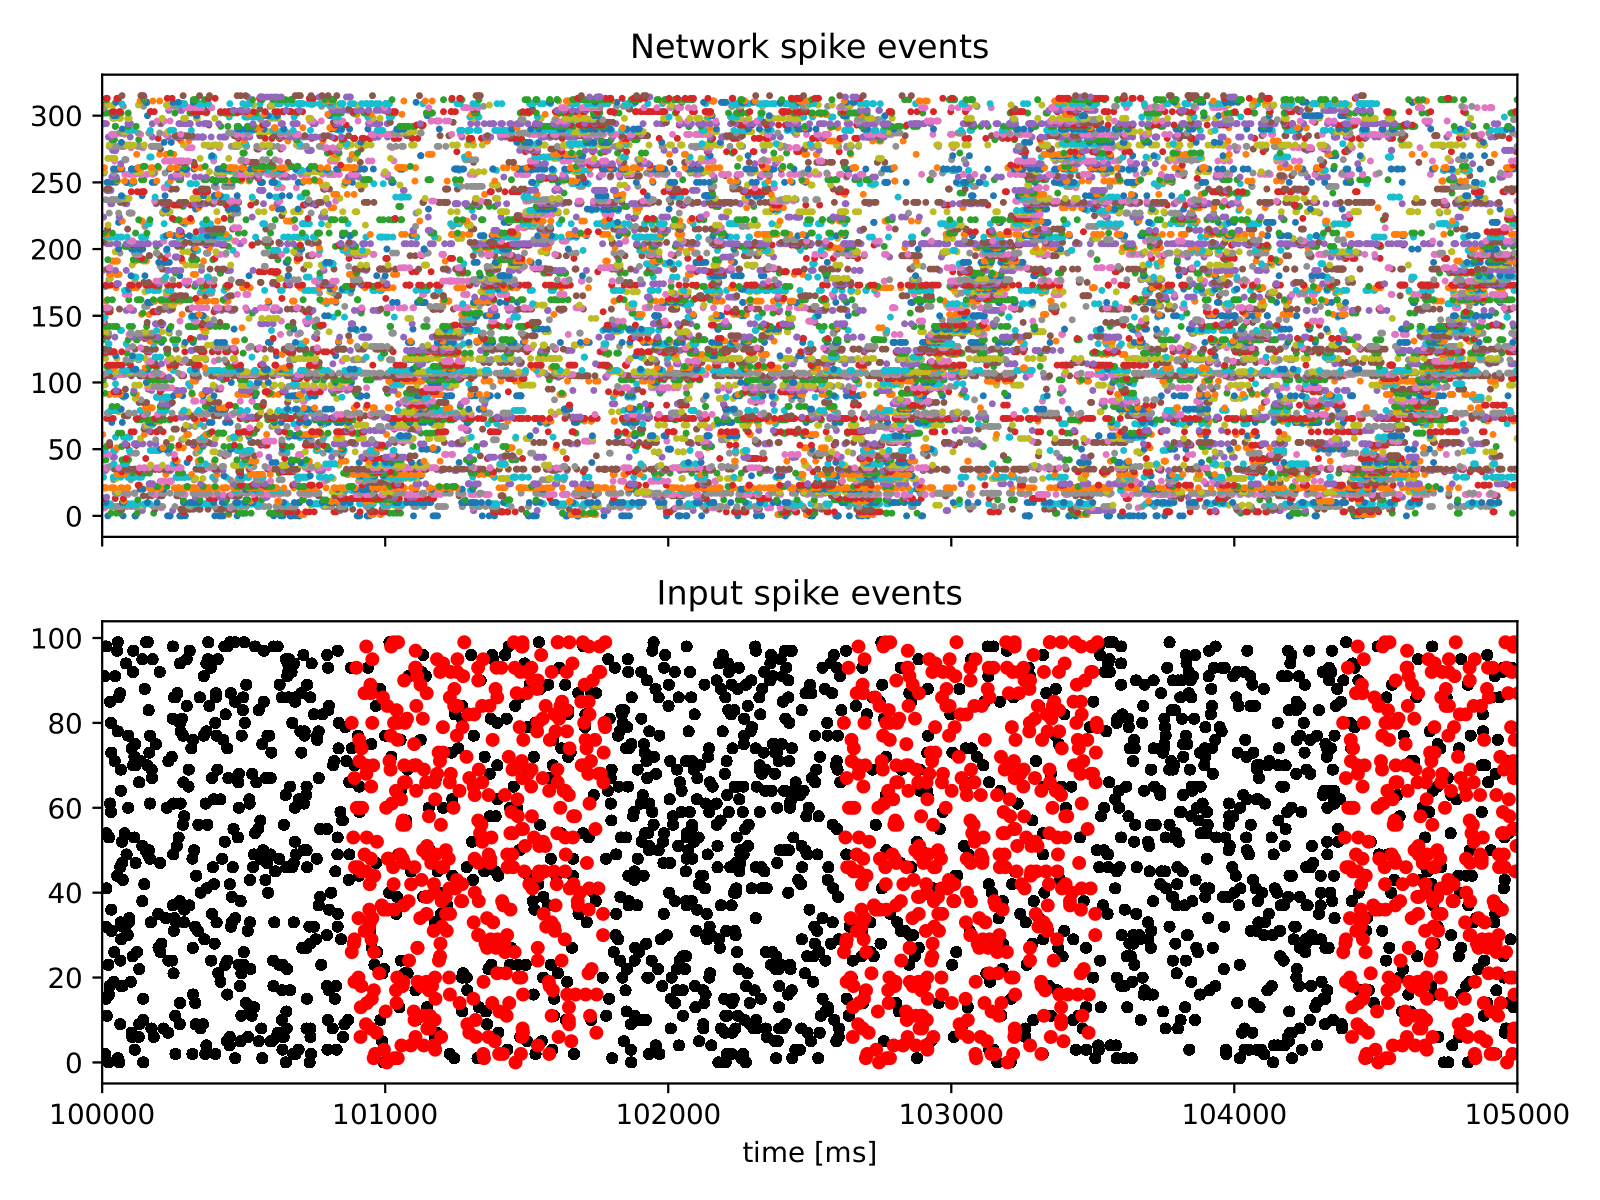
\includegraphics[width=\columnwidth]{Figures/nest_experiment_900ms.png}
    \caption{Pattern duration set to \SI{900}{\milli\second}. Grid size $10\times 5$ with $k\in[2;10]$ and 100 input channels. Input rate of \SI{5}{\hertz} with additional \SI{2}{\hertz} during pattern presentation. \SI{5}{\second} test after \SI{100}{\second} training.}
    \label{fig:nest_experiment_900ms}
\end{figure}






% describe edge case behavior and capabilities of NEST implementation. e.g.:
% prolongated pattern duration (>600ms) to test how much the model can learn
% different patterns



% referring back to the postulated constraint 2. from the Introduction (Chapter \ref{Chapter1}) it is tested if STDP between PCs is needed for required for the formation of spiking assemblies in both the legacy implementation and the new one

